\documentclass[a4paper,12pt]{article}

\usepackage[utf8]{inputenc}
\usepackage[T1]{fontenc}
\usepackage{amsmath,amssymb,amsfonts}
\usepackage{graphicx}
\usepackage[margin=20mm]{geometry}
\usepackage{color}

\newcommand{\todo}[1]{{\color{blue} TODO[#1]}}

\begin{document}

\title{5DV152/VT15: Lab 4}
\author{Christer Jakobsson (870310-8533)}
\date{\today}
\maketitle


\section{Experiment design}
\label{sec:experiment-design}

The experiments where designed in the way that the file \emph{mandel-basic.c} where modified so that there where no image produced. Since the image is not used, the experiments will be done faster if the image isn't made on every repetition. 
Modification where made in the file \emph{common.c}, to be able to get experiment data.
\\\\
For one set of experiments the code were modified so that there where two extra for loops, one to set the environment variable to how many cores should be used. This iterated from 1 to 48 doing runs with different number of cores used.
The other (inner) for loop was used to do repetitions on the calculations 10 times to get more experiment data.\\
\\
So the first experiment where done so that i did ten runs with each number of processors (1 to 48), since there is an implicit barrier at the end of the parallel loops, then printed the time it took for each run and calculated the means and standard deviations with the data i gathered using \emph{octave}.\\
\\
In the second experiment to analyze the load-imbalance, a similar experiment was done, with the difference that \emph{nowait} were used so that the cores did not synchronize after the parallel loops. Each core printed their own execution time.
For each repetition i summarized each threads difference from the thread with max time minus its own execution time.
Then created a list with a sum of the total idle time for each repetition.\\
Then i calculated the mean of all the total idle times and plotted a graph with \emph{errorbars}.
\\The experiment where run with cores 1-48 and 50 repetitions per core.\\
\\For each repetition. \\\emph{sum(maxExectutionTimeInRepetition - coresExecutionTime}\\
\\\\
Paremeters for mandel-basic
\begin{itemize}
\item \emph{Height:} 700
\item \emph{Width:} 600
\item \emph{Pixelsize:} 0.00001
\item \emph{Centerreal:} 0.32
\item \emph{Centerimage:} 0.039
\item \emph{Maxiterations:} 800
\end{itemize}

\section{Results}
\label{sec:results}
Shows the results from the experiments by showing diagrams with calculations from the experiments. 

\subsection{Mean execution times}
\label{sec:exec}
\begin{figure}[h!]
\centering
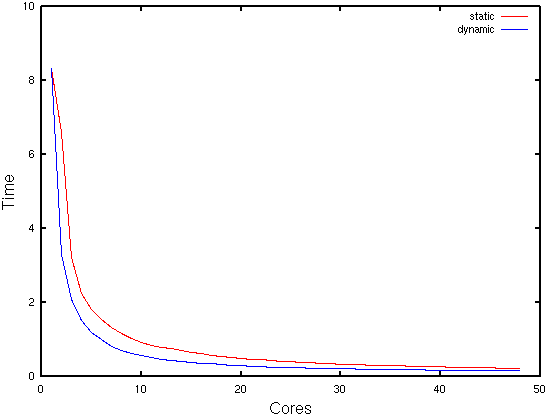
\includegraphics[width=0.6\textwidth]{mean-execution-time-both}
\caption{\emph{Mean execution time: Static and Dynamic scheduling}}
\label{fig:mean-execution-time-both}
\end{figure}

In Figure \ref{fig:mean-execution-time-both} we see that dynamic seems to have a lower execution with number of cores up to 48.

\newpage

\subsection{Mean speed-up}
\label{sec:speed}
\begin{figure}[h!]
\centering
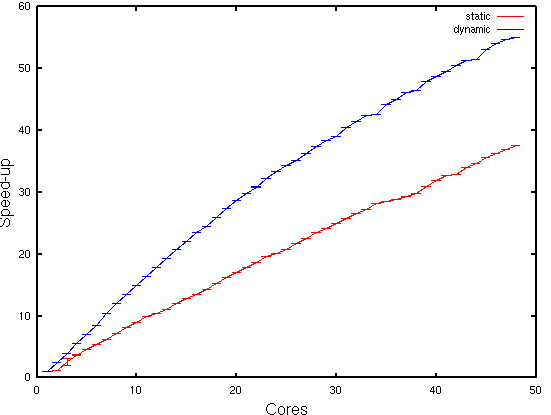
\includegraphics[width=0.6\textwidth]{mean-speed-up-both}
\caption{\emph{Mean speed up: Static and Dynamic scheduling}}
\label{fig:mean-speed-up-both}
\end{figure}

Shows that the curve for both static and dynamic follows the same pattern, but that dynamic have a higher speed-up. 

\newpage

\subsection{Mean load imbalance}
\begin{figure}[h!]
\centering
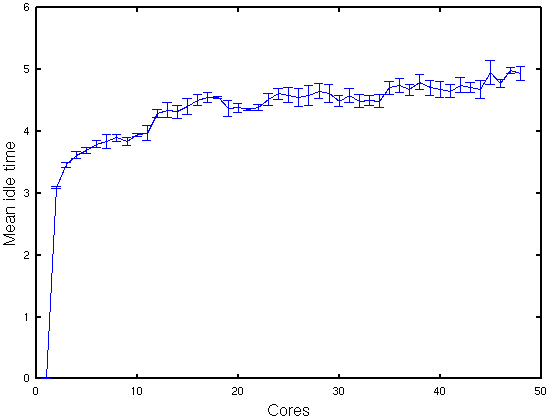
\includegraphics[width=0.6\textwidth]{load-imbalance}
\caption{\emph{Mean idle time, static scheduling}}
\label{fig:load-imbalance}
\end{figure}


\section{Conclusion}
\label{sec:conclusion}
\subsection{Scalability static vs dynamic}
Seen from the graphs in \ref{sec:exec} and \ref{sec:speed} there seems to me that dynamic is in general faster then static scheduling to execute this particular image with the settings i have chosen.
In the aspect of scalability there seems that the speed-up does not converge up-to 48 cores, but the execution time seems to converge with the x-axis at 30 cores.
\\\\
Both static and dynamic scheduling seems to scale good when using many cores, dynamic scheduling scales better seen in \ref{fig:mean-speed-up-both} as its speed-up is more then 50 times with 48 cores,
static scheduling speed-up is at around 35 using 48 cores. Although that dynamic seems to scale better, static does also scale impressively well.
\\\\
\textbf{Static vs dynamic}\\
\begin{tabular}{| l | c | r |}

\hline
  & Static & Dynamic \\ \hline
  Lowest execution times & No & Yes \\ \hline
  Best speed-up & No & Yes \\ \hline
  Converging with x axis? & No & No \\ \hline
\end{tabular}
\\\\\\
Both static and dynamic scheduling does increase in effectiveness when using up to 48 cores,
Although static scheduling seems to lead to higher execution times, from Figure \ref{fig:mean-execution-time-both} there seems like static scheduling is still reaping benefits from using more and more cores, while dynamics execution speed seem to have converged at around 30-40 cores.
This might be because static scheduling is optimized at compile time and therefore utilizes the cores in a more efficient manner when there is many. While dynamic sheduling might lead to poor use of cores since its a out of order, first come first served method.
\\
Dynamic scheduling seems to scale better then static scheduling.

\subsection{Load imbalance}
The load imbalance increases as the number of cores used increases, looking at the graph in Figure \ref{fig:load-imbalance} the total idle time increases much even on a low number of cores. 
There seems like the load imbalance always increases when increasing used cores, which seems likely. Looking at the standard deviations there seems like the idle times for each repetition fluctuates quite much, which means that the work get distributed in a random fashion. 
Giving different total idle times for each repetition. 
\\
My initial thought was that there would be some load-imbalance, but not that there would be this much time wasted as there is. Interesting to see that something is not as optimal as one thinks.
  
\end{document}
